\chapter{Materiales y Métodos}
\label{chap:materiales_metodos}

% ============================================================================
\section{Diseño}
\label{sec:diseno}
% ============================================================================

El estudio emplea un enfoque cuantitativo, observacional y transversal, centrado en un análisis correlacional de los datos registrados por Apple Health durante los últimos 30 días sobre la actividad física (AF) y el comportamiento sedentario (CS), en relación con la percepción de la calidad de vida relacionada con la salud (CVRS) evaluada mediante el cuestionario SF-36. La investigación examina la existencia de relaciones estadísticamente significativas entre los patrones de AF/CS y la CVRS en un único punto temporal, sin incluir un seguimiento longitudinal.

% ============================================================================
\section{Población de Estudio}
\label{sec:poblacion_estudio}
% ============================================================================

La población de estudio estará compuesta por la comunidad estudiantil de la Facultad de Medicina y Ciencias Biomédicas, que asciende a un total de 3340 alumnos, divididos en 2597 de nivel licenciatura (1016 hombres y 1581 mujeres) y 743 de posgrado (374 hombres y 369 mujeres). Esta cifra preliminar incluye posibles candidatos que, de acuerdo con los lineamientos del proyecto, posean un Apple Watch o estén dispuestos a utilizarlo durante el periodo de recolección de datos.

\subsection{Descripción de la Población}
\label{subsec:descripcion_poblacion}

Los estudiantes pertenecen a programas académicos de licenciatura y posgrado, con una distribución mayoritaria en el nivel de licenciatura. La proporción de mujeres supera ligeramente a la de los hombres en ambos niveles de formación. Se consideran aptos para el estudio aquellos individuos que cursan asignaturas en la Facultad y que, por su edad y situación académica, cumplan con las condiciones de inclusión definidas por el protocolo, asegurando representatividad de ambos sexos y de diferentes trayectorias académicas.

\subsection{Criterios de Selección}
\label{subsec:criterios_seleccion}

Los criterios de selección se basarán en la afinidad de los participantes con los requerimientos del proyecto: disponer de un Apple Watch y estar dispuestos a usarlo de manera continua, no presentar limitaciones de salud que impidan su participación, y encontrarse matriculados como estudiantes de licenciatura o posgrado en la Facultad de Medicina y Ciencias Biomédicas. Así mismo, deberán encontrarse en el rango de edad y condiciones clínicas señaladas en el estudio, con el fin de garantizar la confiabilidad de los datos y su pertinencia para el análisis correlacional planteado.

\subsection{Tamaño de la Muestra y Tipo de Muestreo}
\label{subsec:tamano_muestra}

El tamaño de la muestra se determinará tras un sondeo específico para identificar a los estudiantes que cumplan con la posesión o disponibilidad de un Apple Watch, sobre la base de la cifra global de 3340 alumnos. Una vez establecido el número de candidatos potenciales, se definirán los requisitos estadísticos y metodológicos para garantizar la validez del estudio. Se utilizará un muestreo no probabilístico por conveniencia, reclutando a los participantes que cumplan los criterios de selección y expresen voluntariamente su disposición a formar parte del proyecto.

% ============================================================================
\section{Definición Operacional de Variables}
\label{sec:definicion_operacional_variables}
% ============================================================================

\subsection{Relación entre Variables}
\label{subsec:relacion_variables}

La relación de interés en este estudio se centra en analizar si los cambios en los niveles de actividad física (AF) o en el comportamiento sedentario (CS) están asociados con diferencias en la percepción de la calidad de vida relacionada con la salud (CVRS). La hipótesis plantea que un modelo de inteligencia artificial basado en lógica difusa, entrenado con datos biométricos obtenidos de monitores de actividad física portátiles, permitirá predecir con precisión la CVRS en función de los niveles de CS y AF.

Se espera que, a mayor presencia de CS, se observen menores puntuaciones en la percepción de la CVRS, mientras que niveles más altos de AF estarán asociados con puntuaciones más altas en la percepción de la CVRS. Estas predicciones, combinadas con un análisis estadístico basado en los resultados del cuestionario SF-36, buscan identificar correlaciones significativas entre las variables estudiadas, proporcionando evidencia cuantitativa de cómo el CS y la AF influyen en la calidad de vida.

\subsection{Variables Independientes}
\label{subsec:variables_independientes}

Datos cuantitativos del Apple Watch: Número de pasos por día, horas estacionarias, minutos totales en movimiento, gasto calórico activo, frecuencia cardiaca promedio, entre otras.

\subsection{Variables Dependientes}
\label{subsec:variables_dependientes}

\begin{itemize}
    \item Precisión del algoritmo de inteligencia artificial con lógica difusa en la estimación de la categorización de la AF y el CS.
    
    \item Calidad de Vida Relacionada con la Salud (CVRS), medida con el cuestionario SF-36, analizando sus dimensiones (Función física, Rol físico, Dolor corporal, Salud general, Vitalidad, Función social, Rol emocional, Salud mental) y la Puntuación Global.
\end{itemize}

\subsection{Variables de Control}
\label{subsec:variables_control}

Edad, sexo, peso y estatura, entre otras. Se registran para aislar su efecto sobre la asociación AF/CS--CVRS.

\subsection{Operacionalización de las Variables}
\label{subsec:operacionalizacion_variables}

La \Cref{tab:variables_instrumento} presenta las variables recolectadas en el instrumento, las cuales corresponden a la recolección de los datos biométricos obtenidos mediante la selección de características del Apple Health, así como la aplicación del cuestionario de salud SF-36 y su correspondiente puntuación y recodificación de valores obtenidos.

\begin{table}[p]
\centering
\caption{Variables Recolectadas en el Instrumento}
\label{tab:variables_instrumento}
\scriptsize
\begin{longtable}{@{}p{3.5cm}p{2cm}p{2cm}p{2cm}p{4.5cm}@{}}
\toprule
\textbf{Variable} & \textbf{Tipo} & \textbf{Tipo de Variable} & \textbf{Escala} & \textbf{Descripción / Observaciones} \\
\midrule
\endfirsthead
\multicolumn{5}{c}{\tablename\ \thetable{} -- continuación de la página anterior} \\
\toprule
\textbf{Variable} & \textbf{Tipo} & \textbf{Tipo de Variable} & \textbf{Escala} & \textbf{Descripción / Observaciones} \\
\midrule
\endhead
\midrule
\multicolumn{5}{r}{Continúa en la siguiente página} \\
\endfoot
\bottomrule
\endlastfoot
Sexo & Independiente & Categórica & Nominal & Indica el sexo biológico de la persona (p. ej., Masculino / Femenino). \\
\midrule
Edad & Independiente & Numérica & Discreta/Continua & Años cumplidos. Suele considerarse discreta (entera); sin embargo, para algunos análisis se maneja como aproximación continua. \\
\midrule
Peso (kg) & Independiente & Numérica & Continua & Medición del peso corporal en kilogramos. \\
\midrule
Estatura (m) & Independiente & Numérica & Continua & Medición de la talla en metros. \\
\midrule
Número de horas con deambulación & Independiente & Numérica & Discreta/Continua & Horas (o fracción) en las que el usuario registra algún tipo de desplazamiento (de pie, caminando). \\
\midrule
Número horas estacionarias & Independiente & Numérica & Discreta/Continua & Horas (o fracción) en las que el usuario permanece en posición estacionaria. \\
\midrule
Total de horas monitorizadas & Independiente & Numérica & Discreta/Continua & Horas totales en las cuales el Apple Watch registra actividad (pueden ser horas efectivas de uso diario). \\
\midrule
Horas sin registro & Independiente & Numérica & Discreta/Continua & Horas no registradas por el dispositivo (por ejemplo, si el usuario no lo llevaba puesto). \\
\midrule
Minutos totales en movimiento & Independiente & Numérica & Discreta (minutos) & Total de minutos en movimiento (podría convertirse a horas si fuera necesario). \\
\midrule
Total de minutos de ejercicio diario & Independiente & Numérica & Discreta (minutos) & Minutos diarios destinados a actividad física clasificada como ``ejercicio'' (según los criterios del Apple Watch). \\
\midrule
Distancia caminada en kms & Independiente & Numérica & Continua & Distancia recorrida a pie medida en kilómetros (con decimales). \\
\midrule
Número de pasos por día & Independiente & Numérica & Discreta & Conteo total de pasos diarios. \\
\midrule
Frecuencia cardiaca al caminar promedio diario (lpm) & Independiente & Numérica & Continua & Este valor refleja el estado del sistema cardiovascular durante períodos de inactividad o descanso y se considera un indicador clave de la salud general y la condición física. \\
\midrule
Frecuencia cardiaca de reposo promedio diario (lpm) & Independiente & Numérica & Continua & Frecuencia cardíaca de reposo promedio diario. \\
\midrule
Gasto calórico activo (kcal) & Independiente & Numérica & Continua & Estimación del gasto calórico activo según el Apple Watch, en kilocalorías. \\
\midrule
Función física (SF-36) & Dependiente & Numérica (Escala) & Continua & Dimensión del SF-36 (puntaje 0 a 100). Evalúa la capacidad para realizar actividades físicas. \\
\midrule
Rol físico (SF-36) & Dependiente & Numérica (Escala) & Continua & Dimensión del SF-36 que evalúa las limitaciones físicas en la vida diaria. \\
\midrule
Dolor corporal (SF-36) & Dependiente & Numérica (Escala) & Continua & Percibe la intensidad y frecuencia del dolor, afecta la calidad de vida. \\
\midrule
Salud general (SF-36) & Dependiente & Numérica (Escala) & Continua & Percepción global de salud, síntoma de la salud percibida. \\
\midrule
Vitalidad (SF-36) & Dependiente & Numérica (Escala) & Continua & Evalúa energía, fatiga y cansancio. \\
\midrule
Función social (SF-36) & Dependiente & Numérica (Escala) & Continua & Valora el grado de limitación en las relaciones sociales por problemas de salud. \\
\midrule
Rol emocional (SF-36) & Dependiente & Numérica (Escala) & Continua & Evalúa las limitaciones en las actividades diarias por problemas emocionales. \\
\midrule
Salud mental (SF-36) & Dependiente & Numérica (Escala) & Continua & Mide depresión, ansiedad, pérdida de control emocional y bienestar general. \\
\midrule
Puntuación Global (SF-36) & Dependiente & Numérica (Escala) & Continua & Resultado agregado de todos los componentes del SF-36 (promedio final o score total). \\
\midrule
Estimación del algoritmo de lógica difusa & Dependiente & Numérica & Continua & Resultado obtenido por el algoritmo de Inteligencia artificial que integra las características identificadas para el CS y para la AF. \\
\end{longtable}
\end{table}

% ============================================================================
\section{Plan de Análisis Estadístico}
\label{sec:plan_analisis_estadistico}
% ============================================================================

\subsection{Caracterización}
\label{subsec:caracterizacion}

En primer lugar, validaremos el instrumento mediante la revisión de la coherencia interna y la pertinencia de cada ítem; para ello, calcularemos el Alfa de Cronbach y emplearemos el coeficiente V de Aiken con el fin de confirmar la validez de facie y la validez de contenido, cuyas etapas incluyen el diseño, la adaptación, la valoración por expertos y la prueba piloto. Asimismo, describiremos la distribución de las variables a través de frecuencias, medias y desviaciones estándar, con el propósito de identificar posibles valores atípicos, detectar comportamientos anómalos y sentar las bases para el resto de los análisis.

\subsection{Analogía por Atribución (Comparaciones)}
\label{subsec:analogia_atribucion}

A continuación, evaluaremos si existen diferencias significativas entre posibles subgrupos (por ejemplo, sexo o rangos de edad), aplicando pruebas como la t de Student para muestras independientes o ANOVA con comparaciones post hoc (N de Tukey) cuando haya más de dos grupos; esto nos permitirá establecer comparaciones entre distintos niveles o categorías de los participantes y explorar variaciones relevantes de las variables de interés.

\subsection{Relacional (Correlacional)}
\label{subsec:relacional_correlacional}

Posteriormente, verificaremos los supuestos de normalidad y homocedasticidad, para luego realizar correlaciones (Pearson o Spearman) entre las métricas derivadas de la actividad física/conducta sedentaria y las dimensiones del SF-36, con el objetivo de determinar la magnitud y dirección de la relación; en caso de requerir un enfoque explicativo adicional, plantearemos modelos de regresión lineal múltiple que permitan estimar la contribución de cada variable independiente a la variabilidad de la percepción de la calidad de vida relacionada con la salud.

\subsection{Integración}
\label{subsec:integracion}

Finalmente, integraremos los hallazgos en un análisis más avanzado, donde emplearemos un algoritmo de lógica difusa apoyado en las correlaciones y modelos previos, definiendo las reglas de inferencia y las funciones de membresía para capturar la complejidad de la información; de este modo, elaboraremos diagramas y, si es pertinente, un análisis factorial (KMO, varianza total explicada, rotación) que facilite la interpretación integral de los resultados y el desarrollo de conclusiones sólidas sobre la relación entre actividad física, comportamiento sedentario y calidad de vida.

% ============================================================================
\section{Técnicas y Procedimiento}
\label{sec:tecnicas_procedimiento}
% ============================================================================

\subsection{Selección del Dispositivo}
\label{subsec:seleccion_dispositivo}

Para la selección del dispositivo de monitoreo, se utilizó una base de datos detallada que analiza 423 dispositivos de 133 marcas, divididos en 187 monitores de actividad física y 236 relojes inteligentes lanzados desde 2011 \citep{Henriksen2021WearablesPhysicalActivity}. Esta base permitió identificar las capacidades técnicas de cada dispositivo, como sensores incluidos y su utilidad en la medición de patrones de actividad física (AF) y comportamiento sedentario (CS).

\subsection{Análisis de Sensores}
\label{subsec:analisis_sensores}

Del análisis de los 423 dispositivos, se observó que todos cuentan con un acelerómetro, esencial para medir la intensidad y frecuencia del movimiento, lo que facilita la evaluación de la AF \citep{Henriksen2021WearablesPhysicalActivity}. Sin embargo, solo el 38.3\% de los dispositivos (162 de 423) incluyen un sensor de fotopletismografía (PPG), crucial para medir frecuencia y variabilidad cardíaca, indicadores relevantes para evaluar esfuerzo físico y salud cardiovascular \citep{Pinto2023Photoplethysmography}. Aunque en 2011 solo el 14\% de los wearables incluían PPG, esta tecnología creció significativamente, alcanzando un 55\% en los dispositivos lanzados en 2016, lo que refleja su creciente relevancia en la monitorización de la salud \citep{Henriksen2018UsingSmartphone}.

Otros sensores, como el giroscopio (23.9\%) y el GPS (29.6\%), también destacan por su utilidad. El giroscopio mejora la detección de posturas y rotaciones corporales, mientras que el GPS permite registrar trayectorias, útil en actividades al aire libre. Sensores menos comunes, como el magnetómetro (18.2\%) y el barómetro (13.5\%), tienen aplicaciones específicas, pero son menos relevantes para este estudio \citep{Henriksen2018UsingSmartphone}.

\subsection{Elección del Apple Watch}
\label{subsec:eleccion_apple_watch}

El análisis de mercado identificó a Apple como el líder en la categoría de smartwatches, con un 49\% de la cuota global, seguido por Samsung (15\%) y Garmin (11\%) \citep{Canalys2024Smartwatches}. Esta predominancia y la uniformidad en sus dispositivos justifican la elección del Apple Watch como el dispositivo más adecuado, asegurando una mayor representatividad de datos y compatibilidad con herramientas de análisis avanzadas.

\subsection{Protocolo del Instrumento}
\label{subsec:protocolo_instrumento}

Para la implementación del instrumento de realizo un flujo de trabajo como el que se describe en la \Cref{fig:diagrama_flujo}, donde se estableció un protocolo específico para la extracción y procesamiento de variables biométricas obtenidas de dispositivos Apple Watch, utilizando los archivos exportados por la aplicación Apple Health. Este enfoque permitió recopilar las métricas necesarias sin desarrollar una aplicación personalizada ni programar en Swift, garantizando la integridad, y seguridad de los datos a través de un procedimiento manual estructurado que permita su replicabilidad \citep{Apple2024HealthKit}.

\begin{figure}[htbp]
    \centering
    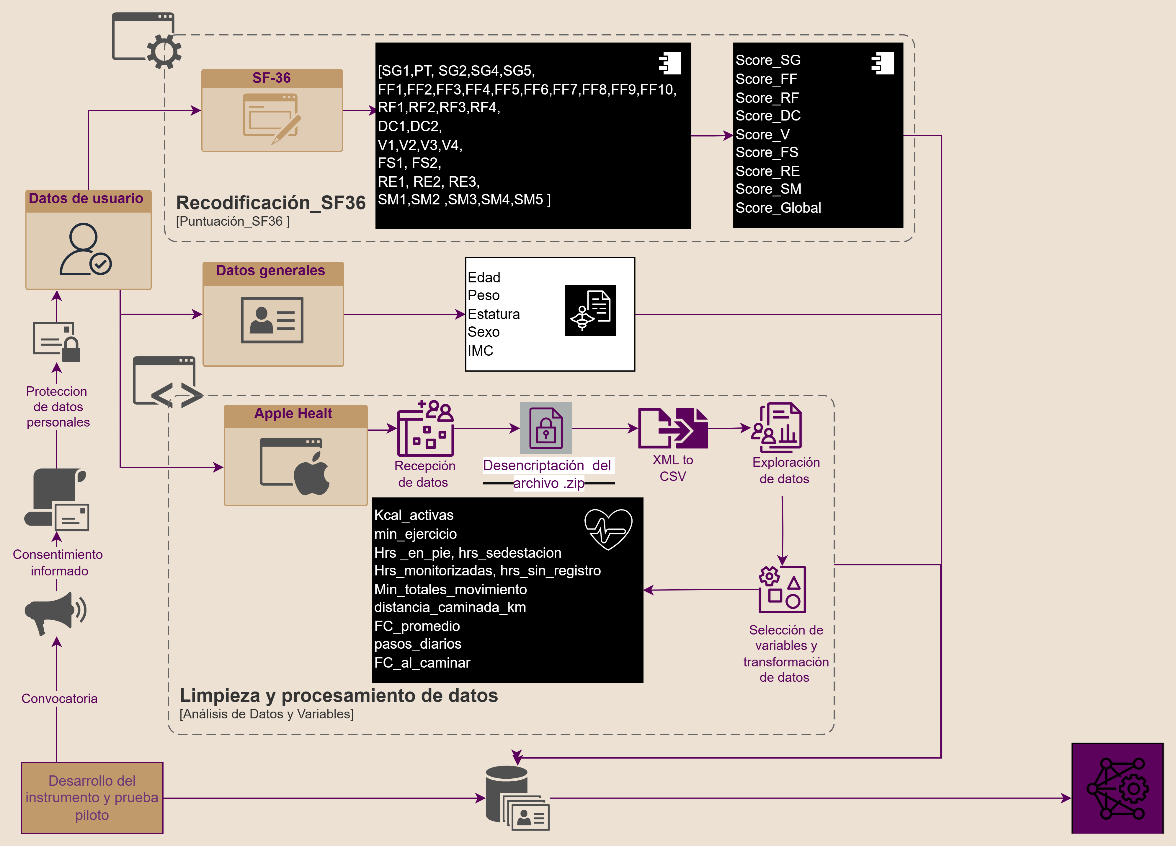
\includegraphics[width=0.9\textwidth]{figuras/diagrama_de_flujo_fig3.png}
    \caption{Diagrama de flujo del proceso de implementación del proyecto de investigación, desde la obtención de datos hasta la selección, extracción, limpieza y procesamiento de las variables}
    \label{fig:diagrama_flujo}
\end{figure}

Recepción y almacenamiento seguro de datos, los participantes generaron un archivo \texttt{export.zip} a través de la aplicación Apple Health en sus dispositivos. Cada archivo fue recibido y almacenado en un entorno seguro, asignándole un código único de participante para asegurar la confidencialidad y trazabilidad de la información. Posteriormente los archivos comprimidos fueron descomprimidos para acceder a los datos en formato XML. Se utilizó el script de código abierto \texttt{apple\_health\_data\_converter.py}, disponible en GitHub, para convertir los archivos XML a formato CSV, facilitando su manejo y análisis estadístico posterior \citep{Gaur2024AppleHealthConverter}.

Se identificaron los archivos \texttt{ActiveEnergyBurned.csv}, \texttt{AppleExerciseTime.csv}, \texttt{AppleStandHour.csv}, \texttt{AppleStandTime.csv}, \texttt{DistanceWalkingRunning.csv}, \texttt{HeartRate.csv}, \texttt{StepCount.csv}, \texttt{WalkingHeartRateAverage.csv} y extrajeron las siguientes métricas específicas relevantes para el estudio \citep{Apple2024HealthKit,Gaur2024AppleHealthConverter}. Posteriormente se desarrolló un código personalizado en Python que requirió de las bibliotecas \texttt{pytz} para el manejo de zonas horarias, \texttt{pandas} para la manipulación de datos y \texttt{numpy} para operaciones numéricas. Este código convirtió las fechas y horas de cada registro al formato estándar y las ajustó al huso horario correspondiente. Para garantizar que los datos provinieran exclusivamente del Apple Watch de cada participante, se filtraron los registros utilizando la columna \texttt{sourceName}. Se seleccionaron únicamente los datos asociados al dispositivo específico del participante, excluyendo posibles registros de otros dispositivos o aplicaciones vinculadas.

Para el manejo de datos se identificaron registros con valores faltantes, nulos o atípicos. Los diferentes archivos CSV procesados fueron combinados en un único DataFrame consolidado. Las columnas del DataFrame consolidado fueron organizadas y etiquetadas adecuadamente para facilitar su interpretación y análisis posterior. Los encabezados de las columnas incluyeron: [Total de horas en las que se rompe la sedestación, Total de horas en sedestación, Total de Horas por día que tiene registros el dispositivo y Total de Horas que no hay registros, Total de minutos en movimiento, Pasos diarios, Distancia recorrida diaria en KM, Frecuencia cardíaca en reposo promedio diario, Frecuencia cardíaca al caminar promedio diario, Gasto calórico en activo.] Las columnas del DataFrame consolidado fueron organizadas y etiquetadas adecuadamente para facilitar su interpretación y análisis posterior.

% ============================================================================
\section{Base Metodológica del Sistema de Inferencia Difusa}
\label{sec:base_metodologica_sistema_difuso}
% ============================================================================

Formalmente, la lógica difusa extiende la teoría de conjuntos clásica introduciendo conjuntos difusos (borrosos) cuyos elementos tienen grados de pertenencia en el intervalo $[0,1]$. Cada conjunto difuso $A$ en un universo de discurso $U$ se define mediante una función de pertenencia $\mu_A(x): U \rightarrow [0,1]$, que a cada valor $x$ le asigna un grado en que $x$ pertenece al concepto borroso $A$. Un grado $\mu_A(x) = 1$ indica pertenencia plena, $\mu_A(x) = 0$ indica no pertenencia, y valores intermedios reflejan pertenencia parcial.

\begin{figure}[htbp]
    \centering
    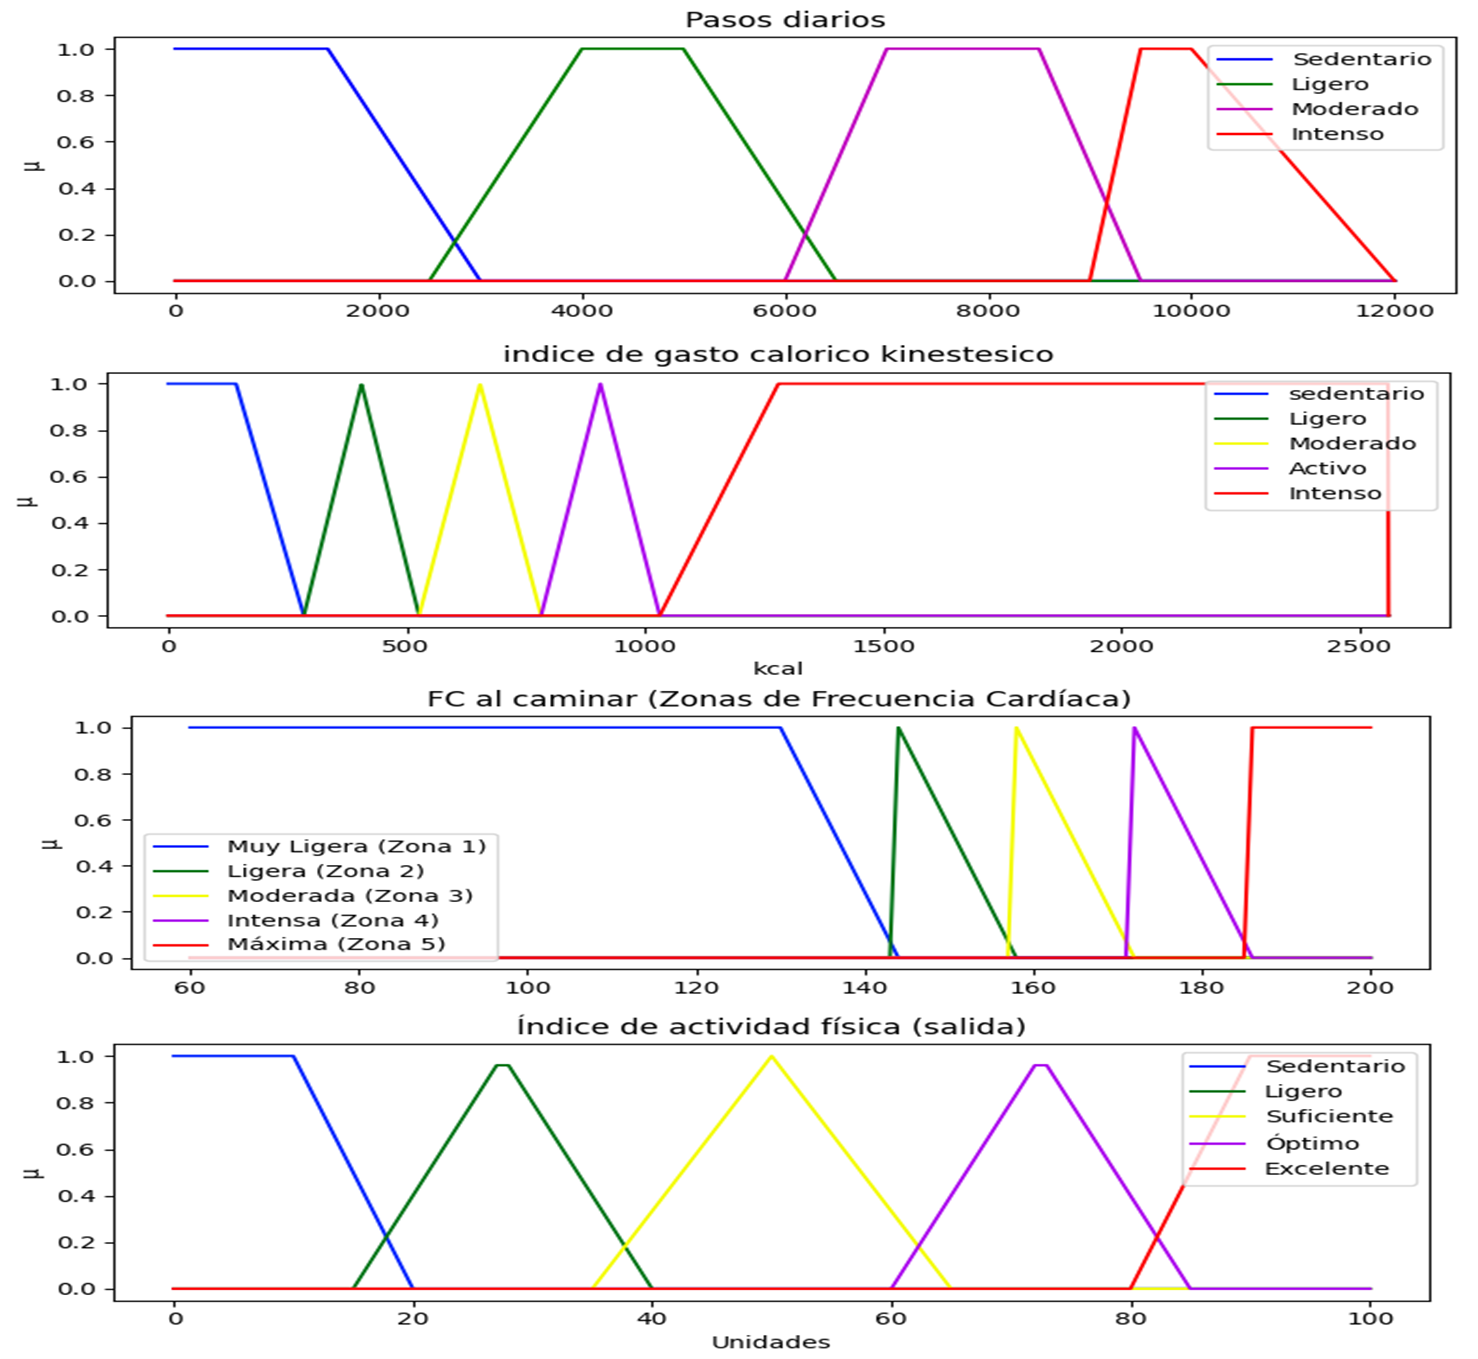
\includegraphics[width=0.95\textwidth]{figuras/Funciones_de_membresias_trapezoidales_fig4.png}
    \caption{Funciones de membresías trapezoidales que representan los universos de discurso: Pasos Diarios, Índice de gasto calórico kinestésico, FC al caminar e índice de actividad física}
    \label{fig:funciones_membresia}
\end{figure}

Por ejemplo, podríamos definir un conjunto difuso ``pasos diarios bajos'' donde $\mu_{\text{bajo}}(x) = 0.8$ para $x = 4000$ pasos, significan que 4000 pasos/día se consideran con un 80\% de pertenencia al concepto ``bajo''. Las funciones de pertenencia típicamente se representan con curvas triangulares, trapezoidales, sigmoides u otras formas, como se observa en la \Cref{fig:funciones_membresia} según convenga modelar gradualmente la transición entre bajo, medio, alto, etc.

Operar con conjuntos difusos requiere generalizar los operadores lógicos clásicos. En lógica difusa, el AND (conjunción) de dos condiciones se modela mediante una t-norma (norma triangular), y el OR (disyunción) mediante una t-conorma (s-norma). Estas operaciones combinan los grados de verdad de los operandos siguiendo ciertas propiedades (conmutatividad, asociatividad, monotonía y existencia de elementos neutro y nulo). La elección más común --por su simplicidad y significado intuitivo-- es usar la mínima (min) como t-norma para AND y la máxima (máx) como s-norma para OR. Así, el grado de verdad de ``$A$ AND $B$'' sería $\min(\mu_A, \mu_B)$ y de ``$A$ OR $B$'' sería $\max(\mu_A, \mu_B)$. De igual forma, la negación (NOT) de un conjunto difuso se define usualmente como el complemento estándar $\mu_{\neg A}(x) = 1 - \mu_A(x)$. Estas operaciones extienden las leyes de De Morgan al caso difuso, permitiendo cálculos lógicos coherentes con valores de verdad parciales.

Con estos elementos, es posible construir reglas difusas del tipo SI-ENTONCES para capturar conocimiento experto. Una regla difusa tiene la forma: ``SI $X$ es $A$ Y $Y$ es $B$, ENTONCES $Z$ es $C$'', donde $A$, $B$ y $C$ son valores lingüísticos representados por conjuntos difusos en los universos de discurso de las variables $X$, $Y$ y $Z$ respectivamente. Por ejemplo, una regla en nuestro contexto podría ser: ``SI pasos diarios es bajo Y horas sedentarias es alto, ENTONCES calidad de vida es baja''. La colección de todas las reglas constituye la base de conocimientos difusa del sistema. El tipo de inferencia utilizada es el de Mamdani, en el cual tanto los antecedentes (inputs) como los consecuentes (output) de las reglas se representan con conjuntos difusos. A diferencia de un modelo Sugeno (que usa salidas crisp definidas por funciones lineales), el modelo Mamdani produce una salida difusa que luego debe convertirse a un valor final preciso mediante defuzzificación como se muestra en la \Cref{fig:salida_difusa}.

\begin{figure}[htbp]
    \centering
    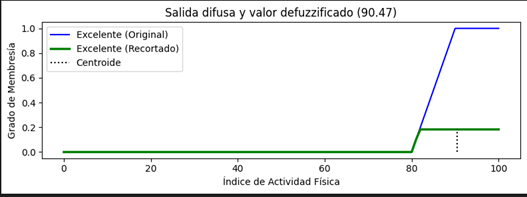
\includegraphics[width=0.85\textwidth]{figuras/Salida_difusa_figura_5.png}
    \caption{Salida difusa del sistema de inferencia donde obtenemos el valor crisp del índice de actividad física resultado del proceso de defuzzificación}
    \label{fig:salida_difusa}
\end{figure}

En resumen, matemáticamente el sistema consta de: (a) conjuntos difusos y funciones de pertenencia que definen las etiquetas lingüísticas para cada variable; (b) operadores lógicos difusos (t-normas, s-normas, negadores) que permiten evaluar la veracidad parcial de premisas compuestas; (c) un conjunto de reglas SI ENTONCES difusas que relacionan las entradas (comportamientos sedentarios/activos) con la salida (impacto en calidad de vida); y (d) un mecanismo de inferencia difusa Mamdani que combina las reglas y obtiene una salida difusa, la cual finalmente se transforma en un valor numérico mediante defuzzificación.

% ============================================================================
\section{Aspectos Éticos y de Bioseguridad}
\label{sec:aspectos_eticos_bioseguridad}
% ============================================================================

Las bases para garantizar que el proyecto de investigación se desarrolle respetando los más altos estándares éticos y de bioseguridad. Al implementar las medidas descritas, se protegerá la confidencialidad y privacidad de los datos de los participantes, cumpliendo con las normativas nacionales e internacionales en cumplimiento con:

\begin{itemize}
    \item Los Principios éticos para las investigaciones médicas en seres humanos de la Declaración de Helsinki.
    
    \item Las Directrices para investigaciones relacionadas con la salud con seres humanos que se establecen en las Pautas Éticas Internacionales del CIOMS.
    
    \item La normativa mexicana para investigaciones en salud que se establecen en el Reglamento de la Ley General de Salud en Materia de Investigación.
    
    \item La legislación mexicana sobre protección de datos personales definida en la Ley General de Protección de Datos Personales en Posesión de Sujetos Obligados.
\end{itemize}

\subsection{Principios Éticos}
\label{subsec:principios_eticos}

El proyecto se regirá por los siguientes principios éticos: \textbf{respeto por las personas}, reconociendo la autonomía de los participantes y protegiendo a aquellos con capacidades disminuidas para tomar decisiones; \textbf{beneficencia}, maximizando los beneficios potenciales y minimizando los riesgos para los participantes; \textbf{no maleficencia}, evitando causar daño innecesario a los participantes; \textbf{justicia}, asegurando una distribución equitativa de los beneficios y cargas de la investigación.

\subsection{Procedimiento para Obtener el Consentimiento}
\label{subsec:procedimiento_consentimiento}

Se proporcionará a los participantes información clara y comprensible que contenga una explicación detallada del estudio, incluyendo objetivos, procedimientos, riesgos y beneficios. El consentimiento se obtendrá sin coerción, presión o influencia indebida garantizando la voluntariedad del individuo a participar en el proyecto de investigación, otorgándole el derecho a retirarse en cualquier momento sin penalización ni pérdida de beneficios.

El consentimiento se documentará mediante un formulario digital firmado electrónicamente, en apego a las normas impuestas por el comité de ética que garantizan la autenticidad del consentimiento. Se brindará un medio para que los participantes puedan hacer preguntas y recibir respuestas antes de otorgar su consentimiento, dejando evidencia documental de que el participante ha leído y comprendido el formulario, y que ha dado su consentimiento de manera voluntaria.

\subsection{Contenido del Formulario de Consentimiento}
\label{subsec:contenido_formulario_consentimiento}

Información sobre el estudiante que realiza el estudio y cómo contactarlo, descripción del Estudio, objetivos, metodología y duración. Procedimientos a detalle de lo que se espera del participante, posibles inconvenientes y ventajas de participar. Medidas de confidencialidad y cómo se protegerán los datos personales, derechos del participante, incluyendo el derecho a recibir respuestas a sus preguntas y a retirar su consentimiento.

\subsection{Evaluación de Riesgos}
\label{subsec:evaluacion_riesgos}

\textbf{Posibles riesgos:} Si los datos personales o de salud son accesados por personas no autorizadas debido a una brecha de seguridad, podría afectar la privacidad del participante. Identificación de participantes: Aun con datos anonimizados, existe el riesgo de que combinaciones de datos permitan identificar a un individuo. Ansiedad o estrés: Reflexionar sobre su salud y comportamiento sedentario podría generar estrés o sentimientos de culpa en algunos participantes. Autopercepción negativa: Los resultados del cuestionario SF-36 podrían afectar la percepción de bienestar si los puntajes son bajos. Dependencia tecnológica: Promover el uso continuo de dispositivos podría incrementar la dependencia en la tecnología. Malinterpretación de datos: Sin una adecuada explicación, los participantes podrían malinterpretar sus datos biométricos, llevando a decisiones inapropiadas sobre su salud.

\textbf{Medidas de Mitigación:} Asegurar la protección de datos, implementado medidas robustas de seguridad para almacenar y manejar los datos. Explicar claramente los posibles riesgos y cómo se pueden manejar, así como ofrecer recursos o referencias en caso de que los participantes experimenten malestar emocional. Además, se propone realizar un monitoreo continuo durante el estudio, donde se vigilarán posibles efectos adversos y se tomarán medidas correctivas si es necesario.

\subsection{Protección de Grupos Vulnerables}
\label{subsec:proteccion_grupos_vulnerables}

Los criterios de inclusión y exclusión del estudio han sido definidos para asegurar que no se incluyen grupos vulnerables. Esto evidencia que se ha considerado su protección y que el estudio ha sido diseñado para minimizar riesgos asociados.

\subsection{Confidencialidad y Privacidad de los Datos}
\label{subsec:confidencialidad_privacidad}

El manejo de los datos personales se basará en los siguientes principios: \textbf{licitud y transparencia}, los datos se recopilarán y procesarán de manera legal y transparente. Se utilizarán únicamente para los fines específicos del estudio limitando la finalidad los datos, solo se recopilarán los datos necesarios y pertinentes, se garantizará que los datos sean precisos y se mantengan actualizados y se protegerán los datos contra accesos no autorizados, pérdidas o daños garantizando la integridad y confidencialidad. Para ello el control de accesos, solo el equipo de investigación tendrá acceso a los datos, y se gestionarán permisos según roles y responsabilidades.

Además, se eliminarán identificadores personales para que los datos no puedan asociarse a individuos específicos, se asignarán códigos únicos a los participantes, manteniendo separados los datos identificativos de los datos de investigación. Para transferencia y comunicación de datos se utilizarán canales de seguros y cifrados. Cuando sea estrictamente necesario el acceso de terceros se firmarán Acuerdos de Confidencialidad para permitir que puedan tener acceso a los datos, garantizando la protección y uso adecuado.

\subsection{Política de Retención y Eliminación Segura}
\label{subsec:politica_retencion}

Los datos personales se conservarán únicamente durante el tiempo necesario para los fines del estudio y respetando las normas interpuestas por el comité de ética.

\subsection{Derechos de los Participantes}
\label{subsec:derechos_participantes}

Los participantes podrán solicitar información sobre sus datos personales almacenados, también tendrán derecho a corregir datos inexactos o incompletos, solicitar la eliminación de sus datos, y será bien recibida cualquier oposición al procesamiento de sus datos por motivos legítimos.

\subsection{Cumplimiento de Normativas y Legislación}
\label{subsec:cumplimiento_normativas}

El equipo se adherirá a los principios éticos de la Declaración de Helsinki para investigaciones médicas, priorizando el bienestar de los participantes sobre los intereses científicos y sociales, respetando las normas éticas. También se cumplirán las pautas éticas internacionales del CIOMS (Consejo de Organizaciones Internacionales de las Ciencias Médicas) que han sido contempladas y declaradas en este documento para salvaguardar los derechos y bienestar de los participantes. Todo esto en acatamiento al reglamento de la ley general de salud en materia de investigación, que solicita el registro del proyecto aprobado por un comité de ética en investigación reconocido.

Además, por la naturaleza de esta investigación nos exime a cumplir también con Ley General de Protección de Datos Personales en Posesión de Sujetos Obligados, donde los participantes en el proyecto serán responsables del manejo adecuado de los datos personales. Se proporcionará un aviso detallado a los participantes sobre cómo se manejarán sus datos las medidas de seguridad implementadas, las medidas técnicas y organizativas para proteger los datos, los criterios de inclusión y exclusión definidos, las instrucciones claras sobre cómo participar y utilizar los dispositivos de monitoreo, el manejo de datos, el análisis de los datos, la divulgación de resultados, intención de publicaciones y si se comparten datos con otros investigadores.

\subsection{Plan de Contingencia y Manejo de Incidentes}
\label{subsec:plan_contingencia}

Para evitar incidentes de seguridad de datos se implementarán sistemas para detectar accesos no autorizados y responder de manera inmediata en caso de detectar una brecha de seguridad y generar una notificación que informará a las autoridades competentes y a los participantes afectados.

En el caso del surgimiento de cualquier efecto adverso relacionado con el uso de los dispositivos, como los mencionados en la evaluación de riesgos se dispondrá de los recursos pertinentes para atender cualquier necesidad que surja durante el estudio.

% ============================================================================
\section{Financiamiento y Lugar Donde Se Realizará El Proyecto}
\label{sec:financiamiento_lugar}
% ============================================================================

El proyecto será financiado con recursos propios, cubriendo los gastos asociados al reclutamiento de participantes, y los costos relacionados con la publicación y difusión de resultados en eventos científicos, según corresponda. Además, se utilizará software libre, específicamente Python y sus bibliotecas (Scikit-learn, Pandas, TensorFlow, y Matplotlib) para la implementación del modelo de IA basado en lógica difusa, análisis de datos biométricos y visualización de resultados.

En cuanto al lugar de ejecución, se llevará a cabo en la Facultad de Medicina y Ciencias Biomédicas, en el laboratorio LIIACOM, donde se dispone de la infraestructura y el acompañamiento académico adecuados para la gestión del proyecto. Esta institución brindará las facilidades de espacio, equipo de cómputo y asesoría necesaria para la realización de las etapas de recolección de datos, validación de instrumentos, análisis estadístico y elaboración de informes científicos.
